% ****** Start of file apssamp.tex ******
%
%   This file is part of the APS files in the REVTeX 4.2 distribution.
%   Version 4.2a of REVTeX, December 2014
%
%   Copyright (c) 2014 The American Physical Society.
%
%   See the REVTeX 4 README file for restrictions and more information.
%
% TeX'ing this file requires that you have AMS-LaTeX 2.0 installed
% as well as the rest of the prerequisites for REVTeX 4.2
%
% See the REVTeX 4 README file
% It also requires running BibTeX. The commands are as follows:
%
%  1)  latex apssamp.tex
%  2)  bibtex apssamp
%  3)  latex apssamp.tex
%  4)  latex apssamp.tex
%
\documentclass[%
 reprint,
%superscriptaddress,
%groupedaddress,
%unsortedaddress,
%runinaddress,
%frontmatterverbose, 
%preprint,
%preprintnumbers,
%nofootinbib,
%nobibnotes,
%bibnotes,
 amsmath,amssymb,
 aps,
%pra,
%prb,
%rmp,
%prstab,
%prstper,
%floatfix,
]{revtex4-2}

\usepackage{graphicx}% Include figure files
\usepackage{dcolumn}% Align table columns on decimal point
\usepackage{bm}% bold math
\usepackage[font=scriptsize,labelfont=bf, justification=justified]{caption}% change fontsize in captions
\usepackage{booktabs}
\usepackage{subfigure}
%\usepackage{hyperref}% add hypertext capabilities
%\usepackage[mathlines]{lineno}% Enable numbering of text and display math
%\linenumbers\relax % Commence numbering lines

%\usepackage[showframe,%Uncomment any one of the following lines to test 
%%scale=0.7, marginratio={1:1, 2:3}, ignoreall,% default settings
%%text={7in,10in},centering,
%%margin=1.5in,
%%total={6.5in,8.75in}, top=1.2in, left=0.9in, includefoot,
%%height=10in,a5paper,hmargin={3cm,0.8in},
%]{geometry}

\begin{document}

\preprint{APS/123-QED}

\title{PHYC40600 - Physics with Astronomy and Space Science Lab 2;\\\vspace{1cm}555 Timer and Raspberry Pi Pico Pulse-Width Modulation}

\author{Daragh Hollman}
\affiliation{%
 daragh.hollman@ucdconnect.ie
}%

\date{\today}% It is always \today, today,
             %  but any date may be explicitly specified

\begin{abstract}
The aims of this report were to explore pulse width modulation (PWM) and its applications through the simulation and construction of several example circuits. These included brightness variations of an LED, a simple digital-to-analogue converter. The 555 timer was also investigated both in PWM and in its application in a time-to-amplitude converter circuit. We attempted to construct this circuit physically, but encountered issues with op-amp integration which could not be resolved due to time constraints.
\end{abstract}

\maketitle

\section{Introduction}

    Pulse width modulation (PWM) is a useful technique for controlling analog circuits digitally. Through the use of high-resolution internal counters, the duty cycle (the ratio of time the signal is on compared to off) of a square wave can be modulated to reduce the average power supplied to a load to a specific analog signal level \cite{barr}. The result is an analogue signal with amplitude at any given time proportional to the width of the pulse. An example PWM signal is shown in figure \ref{fig:PWM} for varying duty cycle. This switching is usually done at high frequencies so no discernible flickering is observed in the power delivery \cite{ucd}.\\

    Applications of PWM begin with simply adjusting the brightness of lights but extend to less obvious use cases such as in the motor power regulation of light rail (such as the LUAS in Dublin \cite{ucd}) and in AM radio transmission \cite{radioworld}.\\

    \begin{figure}
        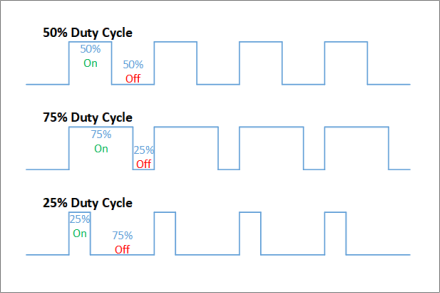
\includegraphics[width=0.9\columnwidth]{Images/pwm.png}
        \caption{\label{fig:PWM}Examples of difference duty cycles for a square wave \cite{ucd}.}
    \end{figure}


\section{PWM with a Raspberry Pi Pico}
The Raspberry Pi Pico is a high-performance microcontroller with multi-function digital I/O pins \cite{Pi, ucd}. PWM is one of these functions. A pin diagram along with full documentation can be found at \url{https://www.raspberrypi.com/documentation/microcontrollers/raspberry-pi-pico.html} \cite{Pi}. For ease of reading, this pin diagram is also included in appendix A.\\

The Pi Pico can be programmed using an implementation of Python 3 designed to run optimally on microcontrollers and other small or otherwise constrained environments called MicroPython \cite{micropython}. MicroPython contains the \textsc{machine} library from which the \textsc{PWM} function can be used to generate a PWM output on a designated pin. The frequency of the PWM can be set up to frequencies beyond $1\,\text{MHz}$, however in this lab we only use up to a maximum $100 \,\text{kHz}$ \cite{ucd}. The duty cycle can be set to an integer value between $0$ and $65535$ (the 16-bit binary maximum), with the ratio of this value and the maximum yielding the ratio the signal will be on compared to off.\\

In this section, we first verify the PWM generation from the Pi Pico behaves as expected, and then design scripts to adjust the brightness of the inbuilt LED on the microcontroller. Following this, the combination of the PWM output and a low pass filter will be used to create a simple Digital-To-Analogue Converter (DAC). Lastly, the generation of analogue signals will be described and demonstrated for a triangle and sine wave.
    
    \subsection{PWM Basics and Applications to Varying LED Brightness}
    To first verify the PWM output from the Pi Pico, a simple script was written to output PWM for a constant frequency and duty. The output of this pin was measured with an oscilloscope and recorded for several duty values with a constant frequency, and also for several frequency values for a constant duty value. Variations in duty are plotted in figure \ref{fig:constFreq}, and variations in frequency are plotted in figure \ref{fig:constDuty}. We can see that the PWM output is what is expected by comparison with figure \ref{fig:PWM}. Frequency adjusts the frequency of the square wave output as a whole, while duty adjusts the amount the square wave is on compared to off.\\

    \begin{figure}
        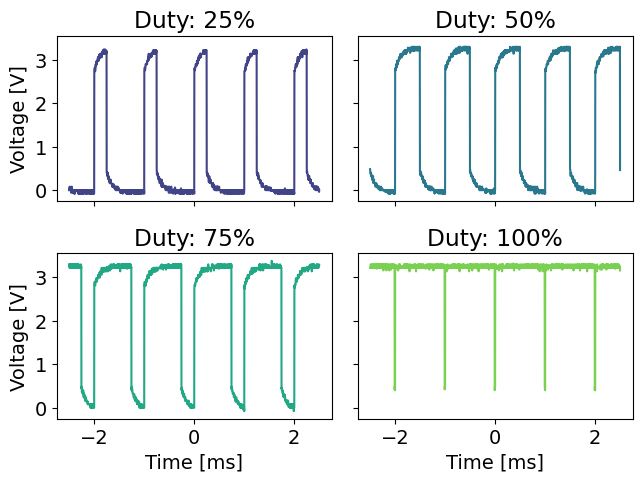
\includegraphics[width=0.9\columnwidth]{Images/constFreq.png}
        \caption{\label{fig:constFreq}PWM output from the Pi Pico showing variations in duty for a constant frequency of $1000 \,\text{Hz}$}
    \end{figure}
    \begin{figure}
        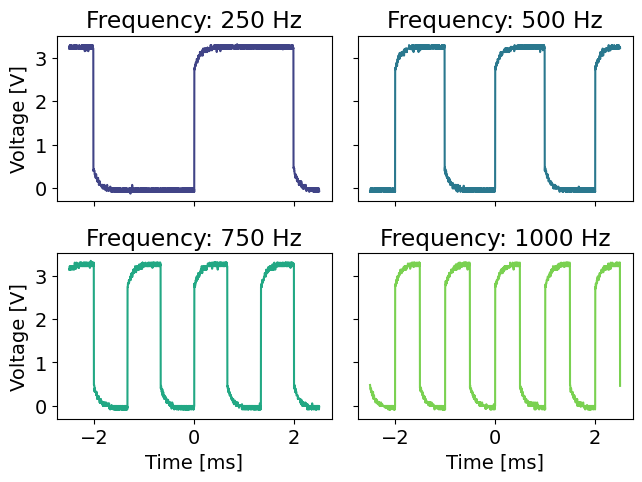
\includegraphics[width=0.9\columnwidth]{Images/constDuty.png}
        \caption{\label{fig:constDuty}PWM output from the Pi Pico showing variations in frequency for a constant duty of $\approx 50$\% (i.e. $65535/2 \approx 32768$, rounding to an integer value.)}
    \end{figure}

    Instead of passing the PWM output to an oscilloscope, the output was sent to internal LED on the Pi Pico (GPIO pin 25, see pin diagram). A \textit{brightness value} float between $0$ (off) and $1$ (full brightness) was defined in the script mentioned previously. The simple multiplication of this brightness value with the maximum duty value $65535$ is sufficient to control the brightness of the LED from this variable. Note that the duty value must be rounded to an integer as this floating point multiplication will result in decimal values which the Pi Pico cannot receive. For low PWM frequencies, flickering of the LED could be observed (as briefly mentioned in the introduction). A 2014 study report that the minimum viewing time required for visual comprehension could be as low as $13\,\text{ms}$ per frame in a sequence \cite{potter_2014}. This corresponds to a minimum frequency $75 \,\text{Hz}$. This value is decisively on the upper end of human capabilities (and is described as such in the study which quotes findings between $13\,\text{ms}$ and $80\,\text{ms}$), given a common monitor refresh rate of $60\,\text{Hz}$ or higher for modern devices \cite{refresh}. To avoid visible flickering in our LED, a higher frequency of $100 \,\text{Hz}$ was chosen.\\

    From here, it is easy to adjust this brightness value over time to linearly transition between $0$ and $1$. A loop was created to increase the brightness in steps of 0.01 for 100 steps, and then decrease again by the same value for a total length of 200 steps. In each step, a small delay $\mathcal{O}(\text{ms})$ could be applied to define the length of time to cycle through the loop. This delay $t_\text{delay}$ was defined as follows:
    \begin{equation}
        t_\text{delay} = \text{round}_\text{ms}\left( \frac{\text{period}}{\text{N}} \right)
    \end{equation}where the period is the length of time for one full cycle, and $N$ the number of steps in the cycle, all rounded to the nearest millisecond.\\

    Observing the LED it is clear that while the brightness value is being incremented linearly, the light does not appear to change linearly in brightness. It appears to stay brighter for longer than it is dimmer. This is however expected, as we know that the human eye has a logarithmic response to changes in light intensity. This phenomenon is part of what is known as the Weber-Fechner Laws \cite{maes_2021}. We can adjust for this, by increasing and decreasing the brightness linearly in log-space. This was not fully achieved for this exercise but a close approximation was implemented which was functionally similar. The brightness was increased with the following equation:
    \begin{equation}
        \frac{10^{t}}{10}
    \end{equation}and decreased with:
    \begin{equation}
        \frac{10^{-(t+1)}}{10}
    \end{equation}where $t$ is the position along the respective half of the 200 step cycle from $0$ to $1$, i.e. $i/100$ where $i$ is the step number. While effective in producing a increase linear in log space, these equations do have the drawback of their bounds. The minimum value, corresponding to $t=0$ for each is only at $10$\% of the maximum brightness, and as such the LED will never reach the fully off state. Despite the constraints on the range, the LED was observed to range between the two brightness values linearly (to the eye). The script for producing both of these effects is included in appendix B.

    
    \subsection{Simple DAC}
    A digital-to-analogue converter (DAC) can be created by passing the PWM output to a low pass filter. The low pass filter acts to attenuate the frequency component of the signal to leave solely the averaged PWM signal as the analogue output \cite{ucd}. The diagram for such a setup is shown in figure \ref{fig:DAC} \cite{ucd}. In a low pass filter the resistance $R$ and capacitance $C$ define the cut-off frequency $f_c$ by the following relation \cite{horowitz}:
    \begin{equation}
        f_c = \frac{1}{2\pi R C}
    \end{equation}At this cut-off frequency, a signal with that frequency has attenuated by $-3 \,\text{dB}$, and further frequencies beyond this cut-off will attenuate at a rate of $-20\,\text{dB}$ per decade. PWM inputs with signal frequencies below this cut-off frequency will be mostly unattenuated and the output will not be smooth. It is then difficult to use high PWM frequencies as the input for the DAC, as larger resistors and capacitors will be needed to increase the cut-off frequency to provide the same attennuating effect.\\

    Given a test input PWM signal of $20\,\text{kHz}$ and a $50$\% duty, a combination of R and C was found to produce a signal with less than $5$\% variation. To achieve this variation, we must first calculate the voltage across the capacitor as it charges as follows:
    \begin{equation}
        V_\text{capacitor} = V_\text{source} \left( 1 - e^{\frac{-t}{RC}} \right)
    \end{equation}where $t$ is the time spent charging with $V_\text{source}$ applied. From here we can solve for a value of RC required. The duty at 50\% will yield an analogue $V_\text{analogue} = 1.65 \,\text{V}$ (half $V_\text{source}=3.3\,\text{V}$), and for this to vary by 5\%, we require:
    \begin{equation}
        V_\text{capacitor} = 1.05 \times 1.65 \,\text{V}
    \end{equation}
    With a charging time per period of $t = \frac{1}{2} \mathcal{T} = 2.5 \times 10^{-5} \,\text{s}$ (for PWM period $\mathcal{T}$), we hence have:
    \begin{align}
        V_\text{capacitor} = \frac{1.05 \times 1.65 \,\text{V}}{3.3\,\text{V}} &= \left( 1 - e^{\frac{-t}{RC}} \right)\\
        0.525 &= 1 - e^\frac{-t}{RC}\nonumber\\
        \frac{t}{RC} &= - \ln(0.475)\nonumber\\
        RC = \frac{t}{0.744} &= 3.36 \times 10^{-5} \,\text{s}
    \end{align}
    While any combination of resistance and capacitance with $RC \ge 3.36 \times 10^{-5} \,\text{s}$ will achieve this, we selected a combination of $R=680\,\Omega$ and $C=1\,\mu\text{F}$, yielding $RC=6.8\times 10^{-4}\,\text{s}$ was chosen based on the components available. This output was verified to have less than 5\% variance using the oscilloscope and the results were plotted in figure \ref{fig:dacVariations}.\\

    It is important that this circuit not be used unbuffered. The output signal from the DAC circuit when connected to another circuit will affect the total resistance of the DAC circuit. The change in RC will cause the cut-off frequency to change, producing an unwanted response from the DAC. This can be amended using a unity gain op-amp to buffer the output signal. A unity gain op-amp is an op-amp circuit which has a voltage gain of 1, meaning the input and output signals are equal voltage \cite{unityGain}. However, one useful property of op-amps for this application is that they typically have very high impedence, and hence, will not draw a significant current from the DAC circuit. The total resistance and hence the RC value will remain unchanged \cite{unityGain}.


    \begin{figure}
        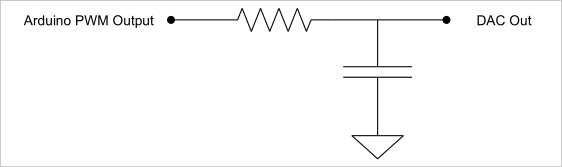
\includegraphics[width=0.9\columnwidth]{Images/dac.png}
        \caption{\label{fig:DAC}A low pass filter to convert the PWM input to an analogue output \cite{ucd}. Note a Pi Pico is used in our case instead of an Arduino, however the principles remain the same.}
    \end{figure}
    \begin{figure}
        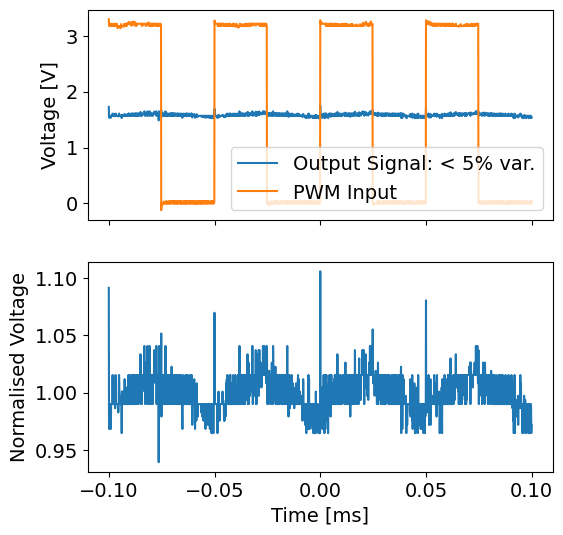
\includegraphics[width=0.9\columnwidth]{Images/dacVariations.png}
    \caption{\label{fig:dacVariations} The output from the simple DAC with a PWM (orange) input of $20\,\text{kHz}$ and $R=680\,\Omega$, $C=1\,\mu\text{F}$ to produce an output signal (blue) with variation less than 5\%. \textit{Second panel}: The DAC output normalised to the mean output.}
    \end{figure}

    \subsection{Generating Analogue Output Functions}
    The combination of the above DAC circuit (to provide an analogue output) and varying the PWM duty cycle (to set the analogue DC level) allows for the creation of specific functions such as a triangular and sine function. This is possible through changing the PWM duty in discrete steps over a cycle \cite{ucd}. A script was written to vary the duty similarly to section II.A., instead this time adjusting the duty according to a custom function for a triangular signal or a sine wave. The full script is available in appendix C.

    \begin{figure*}
        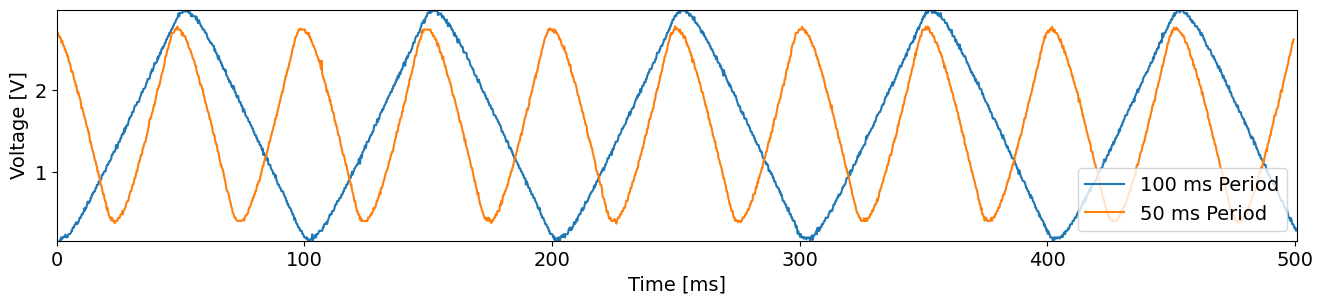
\includegraphics[width=1.8\columnwidth]{Images/triangleFunc.png}
        \caption{\label{fig:triangle}Two triangle functions generated using the combination of PWM and a Low Pass Filter. The period was varied by making a time delay in updating each step of the curve. We note the difficulty in achieving a sharp peak on this function. Higher resistance values in the RC circuit produced sharper triangles, but also resulted in noisier signals.}
    \end{figure*}
    \begin{figure*}
        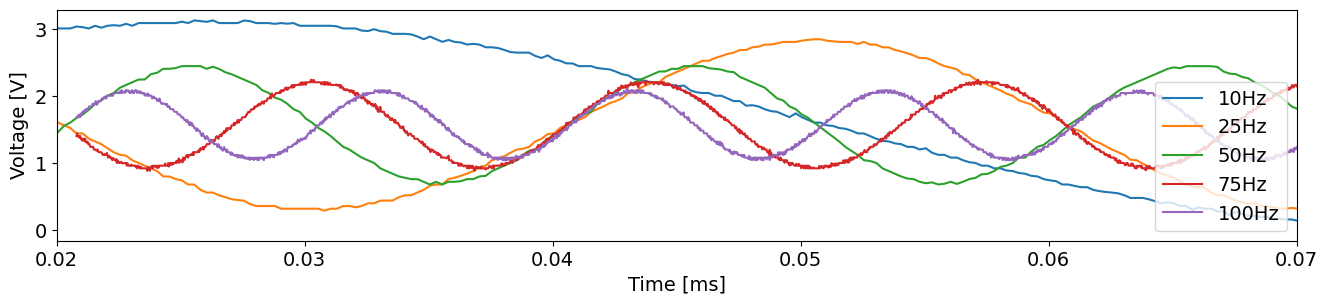
\includegraphics[width=1.8\columnwidth]{Images/sinFunc.png}
        \caption{\label{fig:sin}Several sin functions generated using the combination of PWM and a Low Pass Filter. The frequency was varied with the same method as in the triangle function case.}
    \end{figure*}

        \subsubsection{Triangular Signal}

        A triangular signal was generated through the use of a piecewise function:
        \[T(i) = 
        \begin{cases}
            \frac{2i}{N} & i < \frac{N}{2}\\
            -\frac{2i}{N} + 2 & i \ge \frac{N}{2}
        \end{cases}
        \]
        where $i$ is the step along the function with $N$ steps. The period of the signal was set by applying a short delay along each step of the cycle. This delay was defined as a function of the desired as follows:
        \begin{equation}
            t_\text{delay} = \frac{\text{period}}{N}
        \end{equation}
        Triangle functions for periods of $100\,\text{ms}$ and $50\,\text{ms}$ were plotted in figure \ref{fig:triangle}. We notice that these functions don't peak sharply as expected from the function. Through several observations with varying resistances, we find that higher resistance produces sharper peaks, with the downside of producing more noise on the voltage. For producing these signal functions, we used a $1 \,\text{k}\Omega$ resistor as it provided good signal clarity whilst maintaining minimal noise.

        \subsubsection{Sine Wave}
        
        Sine wave signals were generated similarly, through the use of the following function:
        \begin{equation}
            S(i) = \frac{1}{2}\left(\sin\left(2\pi\frac{i}{N}\right) + 1\right)
        \end{equation}with a frequency set similarly using a delay per time step. Sin functions for frequencies ranging between $10\,\text{Hz}$ and $100\,\text{Hz}$ were plotted in figure \ref{fig:sin}. We notice how the amplitude of each sin wave decreases as the frequency increases, and attempting to generate higher frequency sine waves results in large attenuation. This is expected behaviour, as we expect the low pass filter to attenuate high frequency changes in the input signal. 10 sin waves were generated with frequencies between $1\,\text{Hz}$ to $1\,\text{kHz}$. The amplitude of each sine wave was determined by subtracting the mean value of each wave from the maximum. These values were plotted against their frequency in decibels with respect to the voltage output of the Pi Pico ($3.3\,\text{V}$). See figure \ref{fig:attenuation}. We see the expected response from the low pass filter, with rapid attenuation after the cut-off frequency. This frequency was $f_c = 15.915 \,\text{Hz}$ and is plotted as an orange vertical line through the data. Where it intersects the data is approximately $-1\,\text{dB}$, far from the expected value of $-3\,\text{dB}$. It is clear that the actual cut-off frequency of this circuit must be higher than calculated, potentially due to the use of an unbuffered output affecting the resistance as discussed previously. Tolerance on the components could also play a role but cannot account for the full discrepancy. However regardless, it becomes obvious why high frequency sin waves are being attenuated with this RC configuration.

        \begin{figure}
            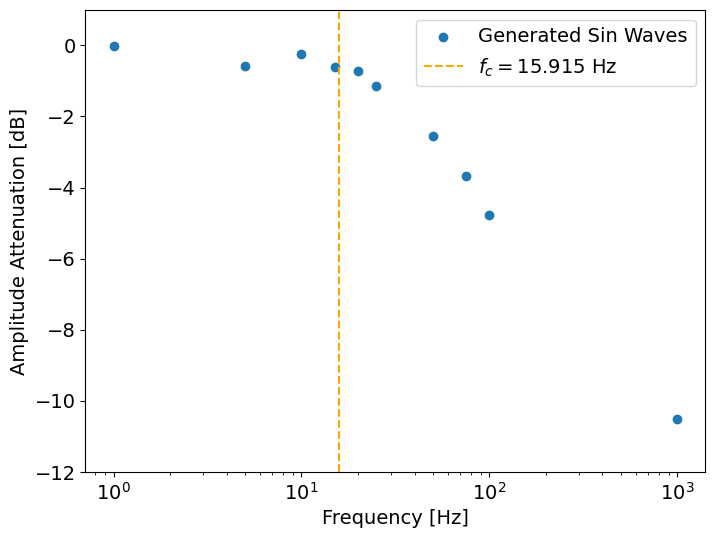
\includegraphics[width=0.9\columnwidth]{Images/attenuation.png}
            \caption{\label{fig:attenuation}The amplitude of the output sin wave plotted with respect to the frequency. We see the typical attenuation curve we expect from a low pass filter. Cut-off frequency (for $R=1\,\text{k}\Omega$ and $C=10\,\mu\text{F}$) is marked by the vertical line.}
        \end{figure}


        \subsubsection{Inaccuracies and Accounting for Processing Time}
        There is an obvious trade-off between increasing the number of steps in the function and time errors in the output. Increasing the number of steps in the function cycle of course increases the accuracy of the output (purely by simply having more data points to plot over the period), however, as Python is by no stretch a slow programming language, we expect delays in the signal output for each step, causing an increase in the overall length of the period. In generating the above functions we initially observed larger periods ($\mathcal{O}(10\,\text{ms})$) than expected. We attempted to ameliorate these errors with a few methods.\\

        While MicroPython contains functions for measuring the time between two points in the code, unfortunately these are not applicable for these purposes as - despite running relatively quickly - take time themselves to run. Hence, they account for the time taken to run the other commands in the loop, but the time they take to run cannot be accounted for.\\

        Another attempt to correct for this issue was to use inbuilt MicroPython function decorators (\textsc{native} and \textsc{viper}). These cause the MicroPython compiler to send to the microcontroller native CPU opcodes in the place of bytecode. These decorators induce limitations on the possible code but generally require no adaptation to the functions \cite{micropython}. The MicroPython documentation suggests these both offer performance increases twice as fast as standard. We were able to implement these decorators however they did not provide improvements significant enough to remove the issue. Difficulties were also encountered with respect to soft restarting the script. We believe the while loop used in the script was not able to be interrupted when converted using these decorators. Fortunately, simply de-powering the Pi Pico by unplugging it fixed these issues.\\

        Other possible implementations include the use of another programming language - C and C++ are approximately 200 times faster than Python in most operations \cite{ucd} - or perhaps the use of third party tools to compile Python to C, see Cython: \url{https://cython.org/}.\\

        The method eventually implemented in the final version of the script was simply a manual correction by visual observation with an oscilloscope. While somewhat crude, it worked effectively and with relatively small errors. As the delay is applied on each step of the function cycle, the correction to the delay must be applied too. Through visual observation, it was quickly apparent that this correction was depended on the number of steps. A table of values was recorded for a range of steps, see table \ref{tab:delayCorrection}. These points were plotted in figure \ref{fig:delayCorrection} and an decaying exponential function was plotted using least squares fitting. A delay correction could be chosen using this function for any given number of steps in the function cycle and applied on each step.

        \begin{table}[]
        \resizebox{0.2\columnwidth}{!}{%
        \begin{tabular}{@{}ll@{}}
        \toprule
        N    & t_c  \\ \midrule
        10   & 900  \\
        15   & 400  \\
        20   & 250  \\
        25   & 150  \\
        100  & 30   \\
        500  & 25   \\
        1000 & 25   \\ \bottomrule
        \end{tabular}%
        }
        \caption{Table of time delay correction values for function generation using the DAC. $N$ is the number of steps in the function cycle, and $t_c$ is the time correction subtracted from the delay in each step.}
        \label{tab:delayCorrection}
        \end{table}

        \begin{figure}
            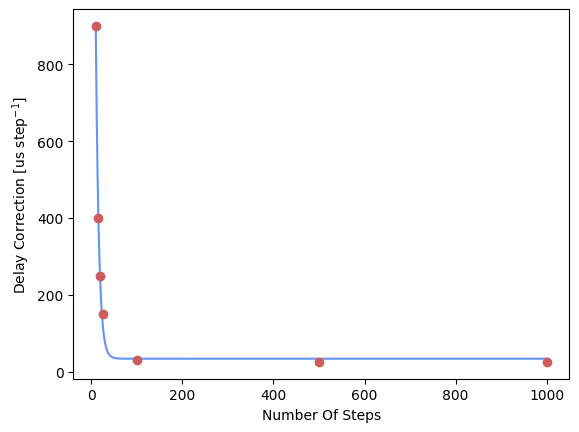
\includegraphics[width=0.9\columnwidth]{Images/delayCorrection.png}
            \caption{\label{fig:delayCorrection}The time correction values from table \ref{tab:delayCorrection} and a least squares exponential fit. This function could then be used to define a time correction for any given number of steps.}
        \end{figure}

\section{555 Timer}
The 555 Timer is a popular integrated circuit chip for timing, a pin diagram is included in figure \ref{fig:555} \cite{horowitz}. The 555 operates in a simple way; It's output is high when the 555 receives a trigger input (trigger pin voltage less than $\frac{1}{3}V_{\text{cc}}$), and goes low when it receives a threshold input (threshold pin voltage higher than $\frac{2}{3}V_\text{cc}$) \cite{horowitz}. When the output is low, the discharge pin connects to ground, and the when the reset pin is low, the output is forced low. The combination of these simple pin functions allows for a large set of complex applications \cite{horowitz}.

\begin{figure}
    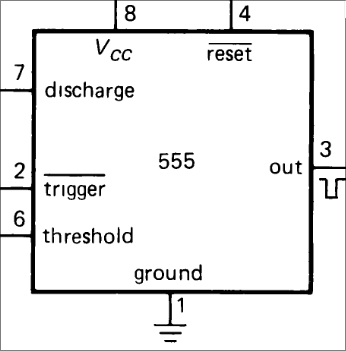
\includegraphics[width=0.7\columnwidth]{Images/555Pins.png}
    \caption{\label{fig:555}A pin diagram for the 555 timing IC \cite{horowitz}. Note, pin 5: Control Voltage is excluded in this diagram.}
\end{figure}
    
    \subsection{555 Timer as an Astable Oscillator}
    Based on the configuration of capacitors and resistors connected to the input pins of the 555, three main operating modes are possible: monostable (creating one fixed-width pulse and returning to stable off), bistable (operating as a flip flop, stable both on and off), and astable (constant oscillations) \cite{555Modes}. In this section, we will explore the functionality of an astable oscillator, see figure \ref{fig:astable}. In this schematic, we see the trigger and threshold pin both connected (through resistors) to $V_{\text{cc}}$. We also see the discharge pin (7) separating this connection. We can infer that as the circuit begins, the $V_\text{cc}$ supply to the threshold will eventually yield the off output from the circuit, however it is slowed by the charging of the capacitor. Until the capacitor is fully charged, the output will be on. However, when the output switches to off, the discharge will be connected to ground, dropping the voltage to the trigger pin, discharging the capacitor and eventually yielding the on output. The astable functionality is created from this repeating cycle \cite{555Modes}.

    \begin{figure}
        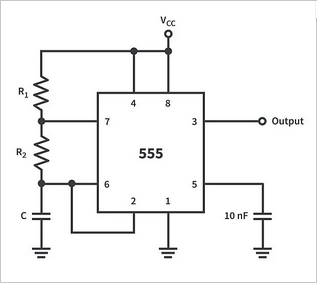
\includegraphics[width=0.9\columnwidth]{Images/astable.png}
        \caption{\label{fig:astable}The configuration of resistors and capacitors required for the 555 to operate in astable mode \cite{555Modes}.}
    \end{figure}

    \begin{figure*}
        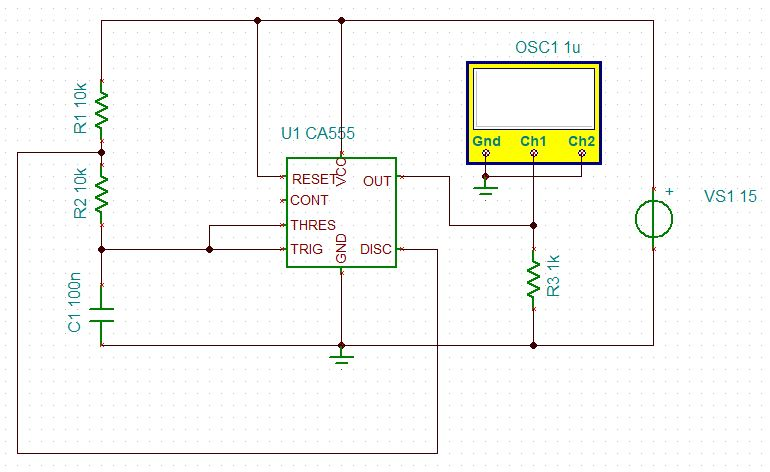
\includegraphics[width=1.4\columnwidth]{Images/astableTina}
        \caption{\label{fig:astableTina}The 555 Timer as an astable oscillator created using Tina \cite{tina}. An oscilloscope is placed at the output of 555 to measure its response.}
    \end{figure*}

        \subsubsection{Simulations}

        \begin{figure}
        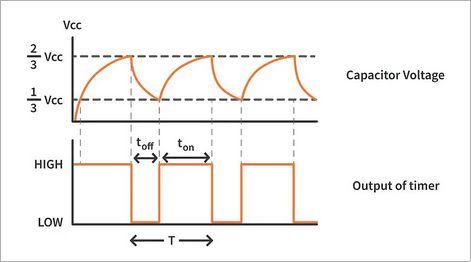
\includegraphics[width=0.9\columnwidth]{Images/astableCapacitor.png}
        \caption{\label{fig:astableCapacitor}How the charging and discharging of the capacitor in the figure \ref{fig:astable} circuit results in differing off and on pulse widths.}
        \end{figure}

        \begin{figure*}
        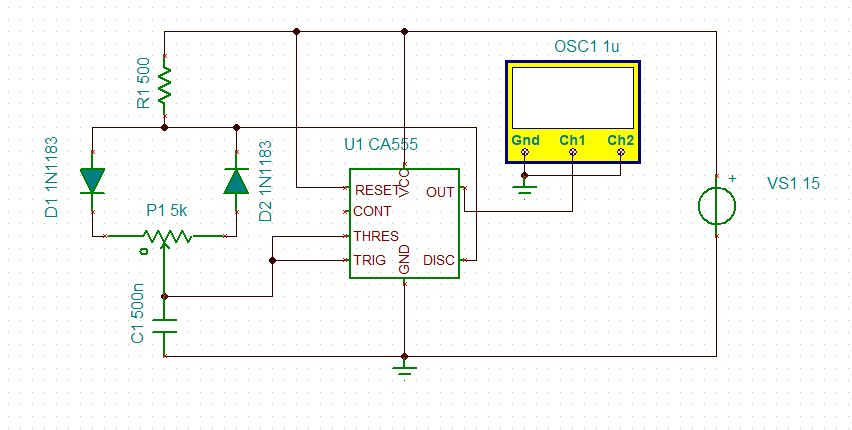
\includegraphics[width=1.6\columnwidth]{Images/potentiometer}
        \caption{\label{fig:potentiometer}The 555 timer in astable mode can be set up using a potentiometer to vary the speed of charging relative to discharging of the capacitor, enabling dynamic PWM \cite{ucd}.}
        \end{figure*}

        \begin{figure}
        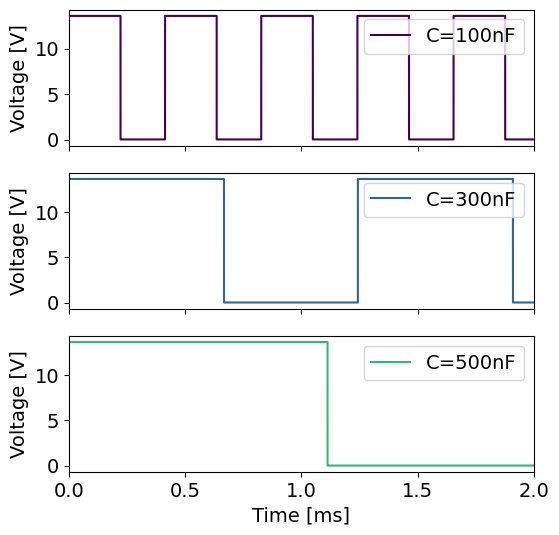
\includegraphics[width=0.9\columnwidth]{Images/potentiometerFrequency.png}
        \caption{\label{fig:potentiometerFrequency}Tina simulations of varying the capacitance in an astable oscillator circuit, see figure \ref{fig:potentiometer}.}
        \end{figure}

        \begin{figure}
        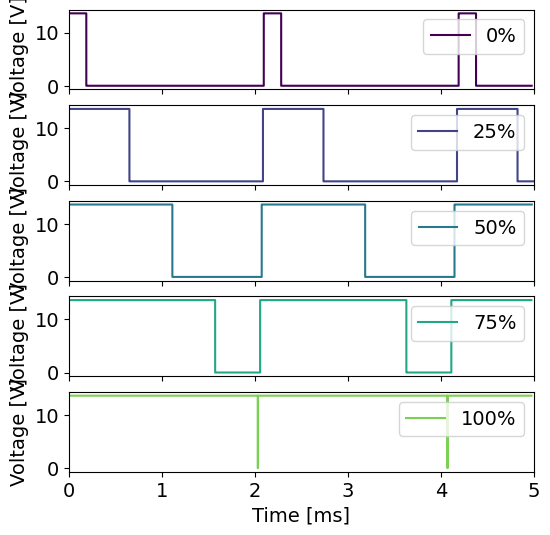
\includegraphics[width=0.9\columnwidth]{Images/potentiometerDuty.png}
        \caption{\label{fig:potentiometerDuty}Tina simulations of varying the charging to discharging rates via a potentiometer in an astable oscillator circuit, see figure \ref{fig:potentiometer}. We see a linear mapping of potentiometer value to duty.}
        \end{figure}

        We performed simulations of the 555 timer as an astable oscillator using TINA \cite{tina}. The circuit was set up as shown in figure \ref{fig:astableTina}. We observe that while the charging of the capacitor is dependent on both  resistors (as both are between it and $V_\text{cc}$), the discharging only has to flow through one of the resistors. Hence, we can vary the values of each resistor to vary the length of time the 555 is on compared to off. We also find we can vary the overall frequency of oscillations by changing the capacitance so that the capacitor charges and discharges slower or faster. An example of this varied charging and discharging looks like is shown in figure \ref{fig:astableCapacitor}. We can see how changing these resistor values effectively changes the duty of a PWM signal as shown in previous sections.\\

        This PWM feature can be shown more clearly through the use of a potentiometer to vary resistance of one of the previous resistors. A circuit to demonstrate this was simulated in Tina as shown in figure \ref{fig:potentiometer} \cite{tina}. This circuit was simulated for different potentiometer resistances and capacitors to fully demonstrate the functionality of the circuit. Figure \ref{fig:potentiometerFrequency} shows simulation outputs showing how changing the value of capacitance will affect the frequency of oscillations in the output. Figure \ref{fig:potentiometerDuty} shows simulation outputs showing how changing the value of the potentiometer affects the duty cycle of these oscillations. We see that the use of diodes in the circuit allows for the mapping of equal resistances to the 50\% point of the potentiometer. We also see that for a potentiometer value of 0\%, we still have an on signal for an appreciable portion of the cycle. This likely due to non-zero resistance minima in non-ideal potentiometers. The weight of this effect can be mitigated by increasing the size of the other resistor between the potentiometer and $V_\text{cc}$, causing the on signal width to be smaller relative to the off signal width.


        \subsubsection{Circuit Construction}
        This circuit was then constructed following the diagram in figure \ref{fig:potentiometer}. A $5\,\text{V}$ external power supply was used to supply the $V_\text{cc}$ and a simple motor was used to load the circuit. The output of the 555 was passed to the base of a transistor allowing current to flow from the power supply through the motor to ground. This circuit was tested for different RC values. As expected, we found that by varying the potentiometer value, the power to the motor changed and it spun faster or slower. By varying the capacitance in the circuit, the frequency of the 555 output could be changed. The motor response was predominantly the same regardless of frequency, with the most noticeable difference being in the audible tone the motor produced changing in pitch. We encountered a large inertial resistance to spinning (the motor could first be set to higher potentiometer values to get the motor spinning before returning to the target speed), which seemed to be - while somewhat difficult to notice - more difficult to overcome with higher frequency outputs.


    \subsection{Designing a Time-To-Amplitude Converter utilising the 555 Timer}

        \subsubsection{Theory}
        A time-to-amplitude converter (TAC) is a device capable of precisely measuring small time intervals and outputting a pulse with proportional amplitude \cite{ortec}. The TAC is an important tool with applications in nuclear physics for measuring the decay times of a short-lived particle (such as in measuring muon lifetimes) \cite{horowitz, muons}.\\

        A simple circuit example of a TAC is included in figure \ref{fig:tacManual} \cite{ortec}. A source of constant current is used to charge a capacitor linearly (limited by saturation) by the following relation:
        \begin{equation}
            V = \frac{I t}{C}
        \end{equation}where $V$ is the voltage across the capacitor, $I$ is the constant current, and $t$ the time \cite{ortec}. After receiving a start signal, the "start" switch opens and "stop" switch closes allowing the capacitor to start charging. The "stop" switch subsequently closes on a stop signal and the voltage built up on the capacitor is gives the amplitude for the output signal. On a stop signal, the linear gate opens to pass the voltage pulse out, and then closes after some time resulting in a fixed width rectangular pulse output \cite{ortec}. The capacitor is then discharged and switches are all returned to their initial positions.\\

        \begin{figure*}
            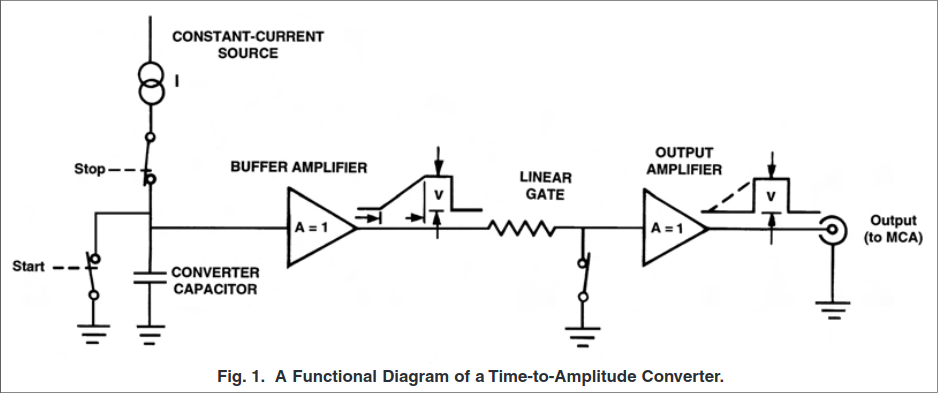
\includegraphics[width=1.8\columnwidth]{Images/tacManual}
            \caption{\label{fig:tacManual}A simplified example of a TAC circuit \cite{ortec}. Note that toggle switches have been included for simplicity, and TAC circuits generally use transistors as switches for such actions \cite{ortec}.}
        \end{figure*}
        
        \begin{figure*}
            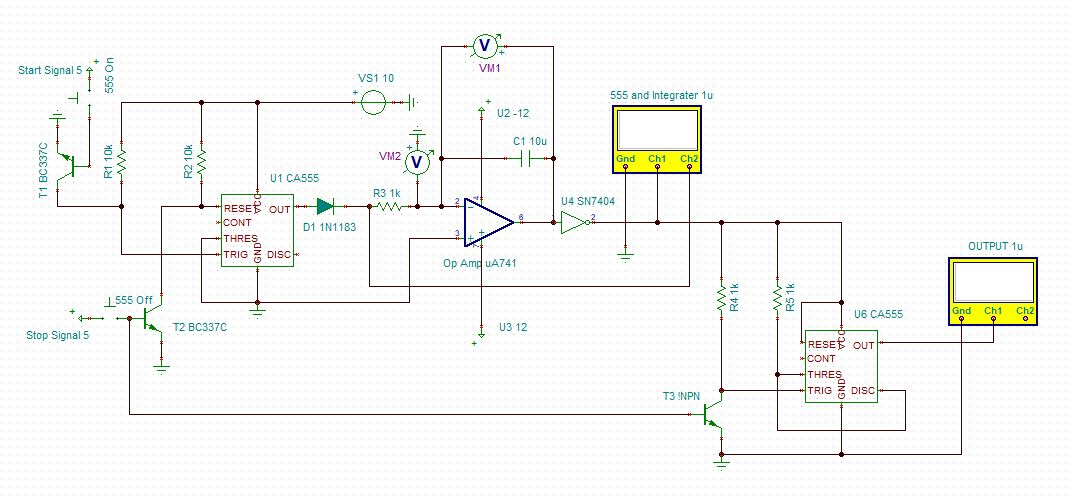
\includegraphics[width=2\columnwidth]{Images/tac}
            \caption{\label{fig:tac}A full circuit diagram for the TAC simulation in Tina.}
        \end{figure*}

        While a simple representation, some of these components - namely the constant current source - are non-trivial to construct in a undergraduate lab environment. However, it should also be possible to recreate the functionality of this circuit (at least as a proof of concept) using a bistable 555 timer and an integrating op-amp.

        \subsubsection{Bistable 555 Timer}
        Discuss what it is, what is different from the astable. Include simple circuit diagram. Explain how the start and stop signals can power transistors to switch on and off.\\

        A 555 timer in bistable mode differs from the astable mode described about in that both the on and off outputs are stable. The 555 effectively acts as a switch and remains in the on or off state as desired. The circuit diagram of the bistable 555 can be found on the left side of figure \ref{fig:tac}. The leading edge of the start signal will apply a voltage to the base of a transistor, grounding the trigger and causing the 555 output to turn on. Similarly, a stop signal grounds the reset pin via a transistor causing the 555 output to be low. Hence, for the time between the leading edge of the start and stop signals, the 555 output will be high, after which it is low.

        \subsubsection{Integrating Op Amp}
        The output of the 555 is passed to an integrating op-amp. Op-amps allow for nearly perfect integrators, without the restriction of the output voltage being less than the input \cite{horowitz}. The integrator adds the signal from the inverting input by charging a capacitor in the feedback loop. The voltage of the capacitor with respect to the non-inverting input is then given by the following equation \cite{horowitz}:
        \begin{equation}
            V_\text{out} = -\frac{1}{RC} \int V_\text{in} dt + \text{const.}
            \label{eq:integrator}
        \end{equation}where $R$ and $C$ are the resistance and capacitance of the integrator circuit and $V_\text{in}$ is the voltage input. This voltage level can then be passed to any means of generating a pulse. The op-amp circuit in our TAC can be found in the centre of figure \ref{fig:tac}.

        \subsubsection{Monostable 555 Timer}
        To create the pulse, a monostable 555 Timer was used, see the right hand side of figure \ref{fig:tac}. A monostable 555 is constructed such that it creates a single fixed with pulse after grounding the trigger pin which has an amplitude equal to the $V_\text{cc}$. By passing the integrated voltage to the $V_\text{cc}$ when a stop signal arrives, an output pulse with fixed width can be created by grounding the trigger.\\

        The circuit as a whole then works in the following way. The start pulse arrives and grounds the trigger pin causing the output of the bistable 555 to go high. As a result, the input of the op-amp integrator is high and the capacitor starts charging as the op-amp integrates the 555 signal. When a stop signal arrives, the monostable 555 is reset and the output goes to off. The op-amp stops integrating further and a fixed with output pulse is created by the monostable 555, with amplitude proportional to the capacitor voltage, and hence, proportional to the time between the stop and start signals.\\ 

        \subsubsection{Testing}

        The circuit was simulated using Tina and some unexpected behaviour occurred. Unwanted capacitor charging and discharging was occurring in the Tina simulations of the circuit. A diode was included between the bistable 555 output and the integrator input to ensure no discharging could occur back through the 555. Other diode positions were tried with respect to the integrator but this position yielded expected output. A voltage inverter was used after the integrator. As shown in equation \ref{eq:integrator}, the voltage output from the integrator is negative with respect to the input, and hence must be inverted to restore a positive voltage signal passed to the monostable 555. The circuit was difficult to demonstrate using Tina as - shown in figure \ref{fig:tac} - push buttons were used to generate start and stop signals and hard to create consistency in inputs. Larger $R$ and $C$ values were used to slow the integration time to measure these longer time intervals.\\

        We attempted to construct this circuit physically but unfortunately could not get it functional for manual signal inputs. The bistable 555 timer and transistor switches were implemented and functional, however, adding the integrating op-amp to the circuit proved non-trivial. Despite trying many configurations and thorough troubleshooting (limited due to time constraints) the integrator output remained at $\approx0\,\text{V}$ regardless of bistable 555 input.\\

        \subsubsection{Configuration}
        Should the circuit have worked as expected, several steps would need to taken to convert from a simple proof of concept to a practical device. Primarily, component values must be selected to map integration time to a chosen range of times - i.e. the millisecond range, or microsecond range - for a given amplitude range. The output pulse generation method we use restricts the integrated voltage between $5\,\text{V}$ and $15\,\text{V}$ due to limits on the 555 timer \cite{555Modes}. This can be done through the use of equation \ref{eq:integrator} as the voltage output of the integrator is inversely proportional to the RC value. The $V_\text{cc}$ voltage of the bistable 555 also plays a roll in the speed of integration. Other useful functionality would be in the adjustment of the output pulse, specifically its width. This could be varied by switching resistance values in the monostable 555 circuit.\\

\section{Conclusions}

Pulse width modulation and its applications were investigated and explored through the use of several examples including brightness variations of an LED, a simple digital-to-analogue converter, and the 555 timer. We also showed an example application for the 555 timer in a time-to-amplitude converter circuit. This circuit is explained in detail along with steps for configuration, and was simulated using the Tina circuit simulator. We attempted to construct this circuit physically, but encountered issues with the op-amp integrator and could not resolve them due to time constraints.
    

\bibliographystyle{unsrt}
\bibliography{aps_references}% Produces the bibliography via BibTeX

\clearpage
\onecolumngrid
\appendix

\section{Pi Pico Pin Diagram}

    \begin{figure}[h]
        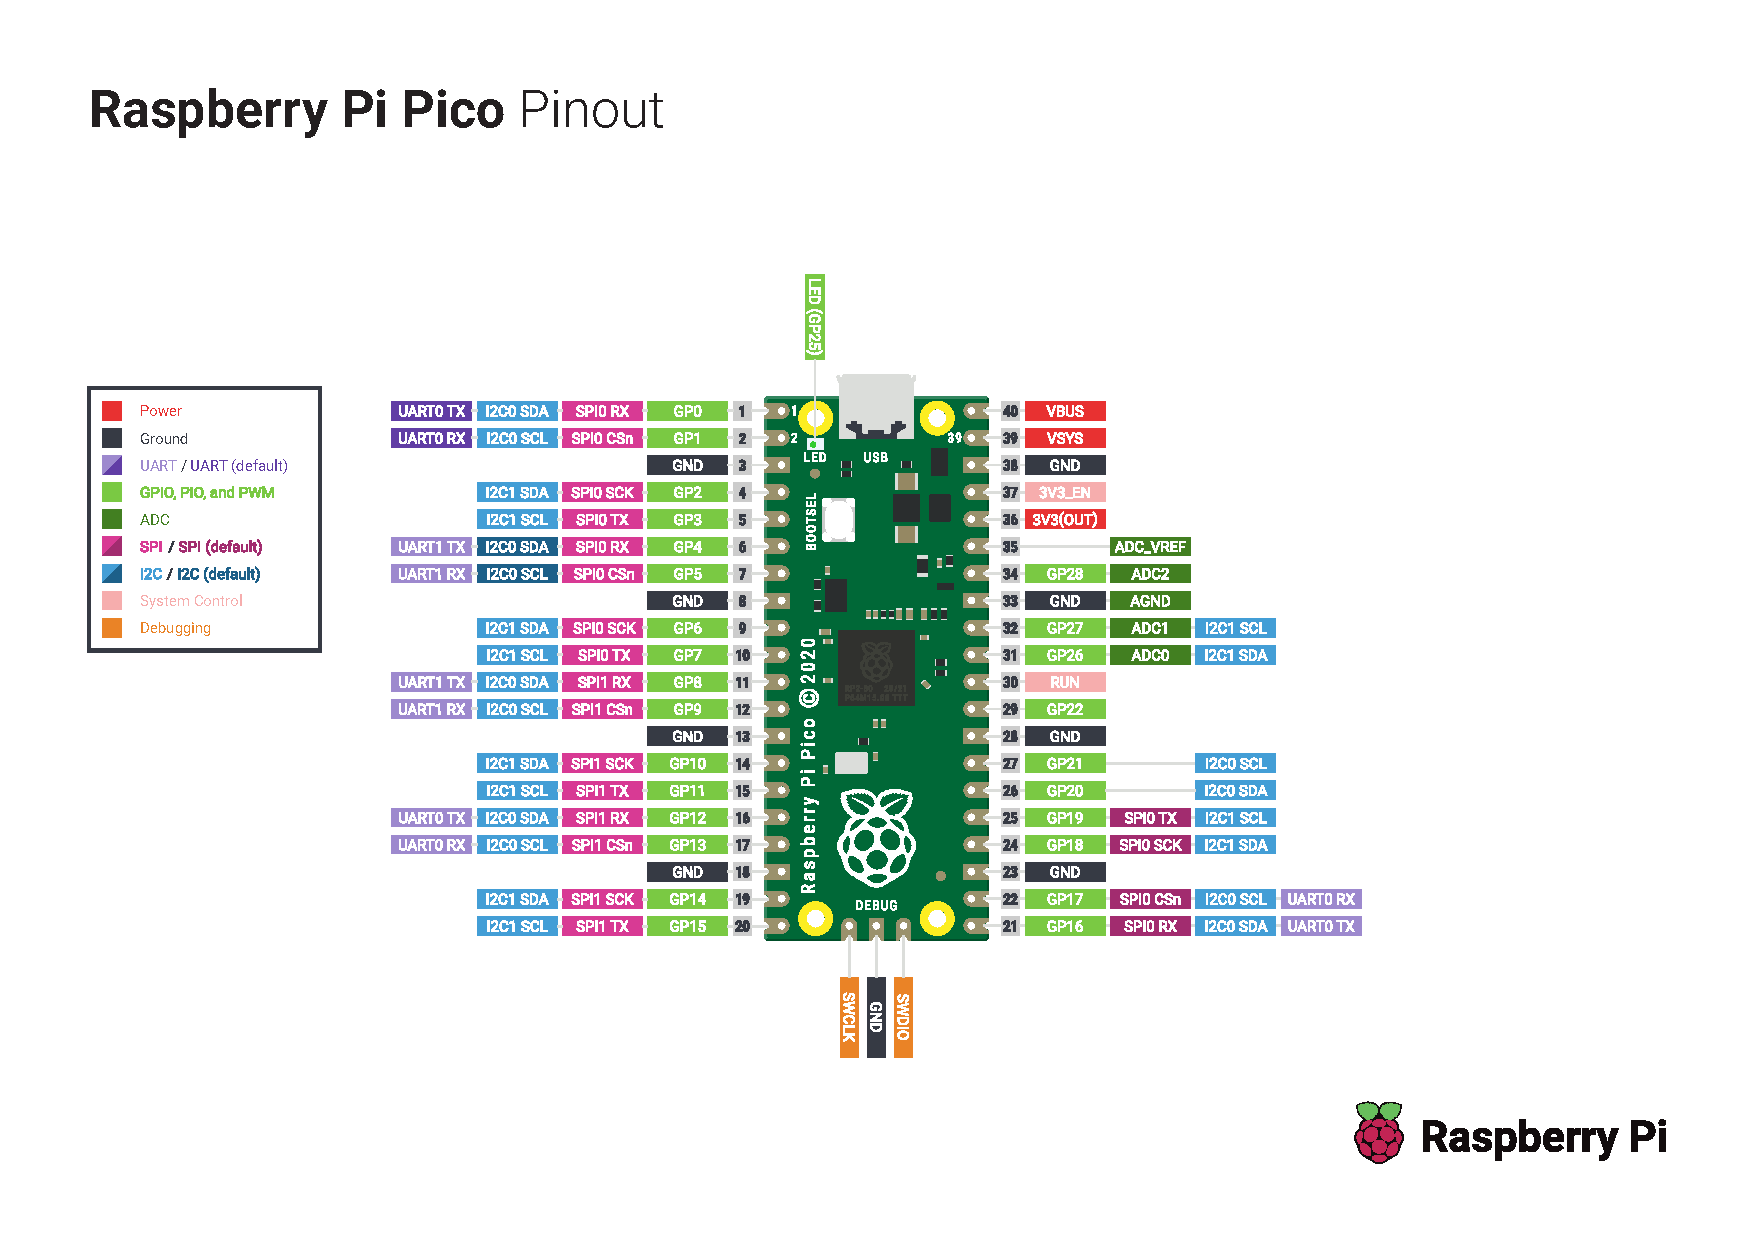
\includegraphics[width=\columnwidth]{Images/Pico-R3-A4-Pinout.pdf}
    \end{figure}

\section{Linear / Log Brightness Script}
    \begin{figure}[h]
        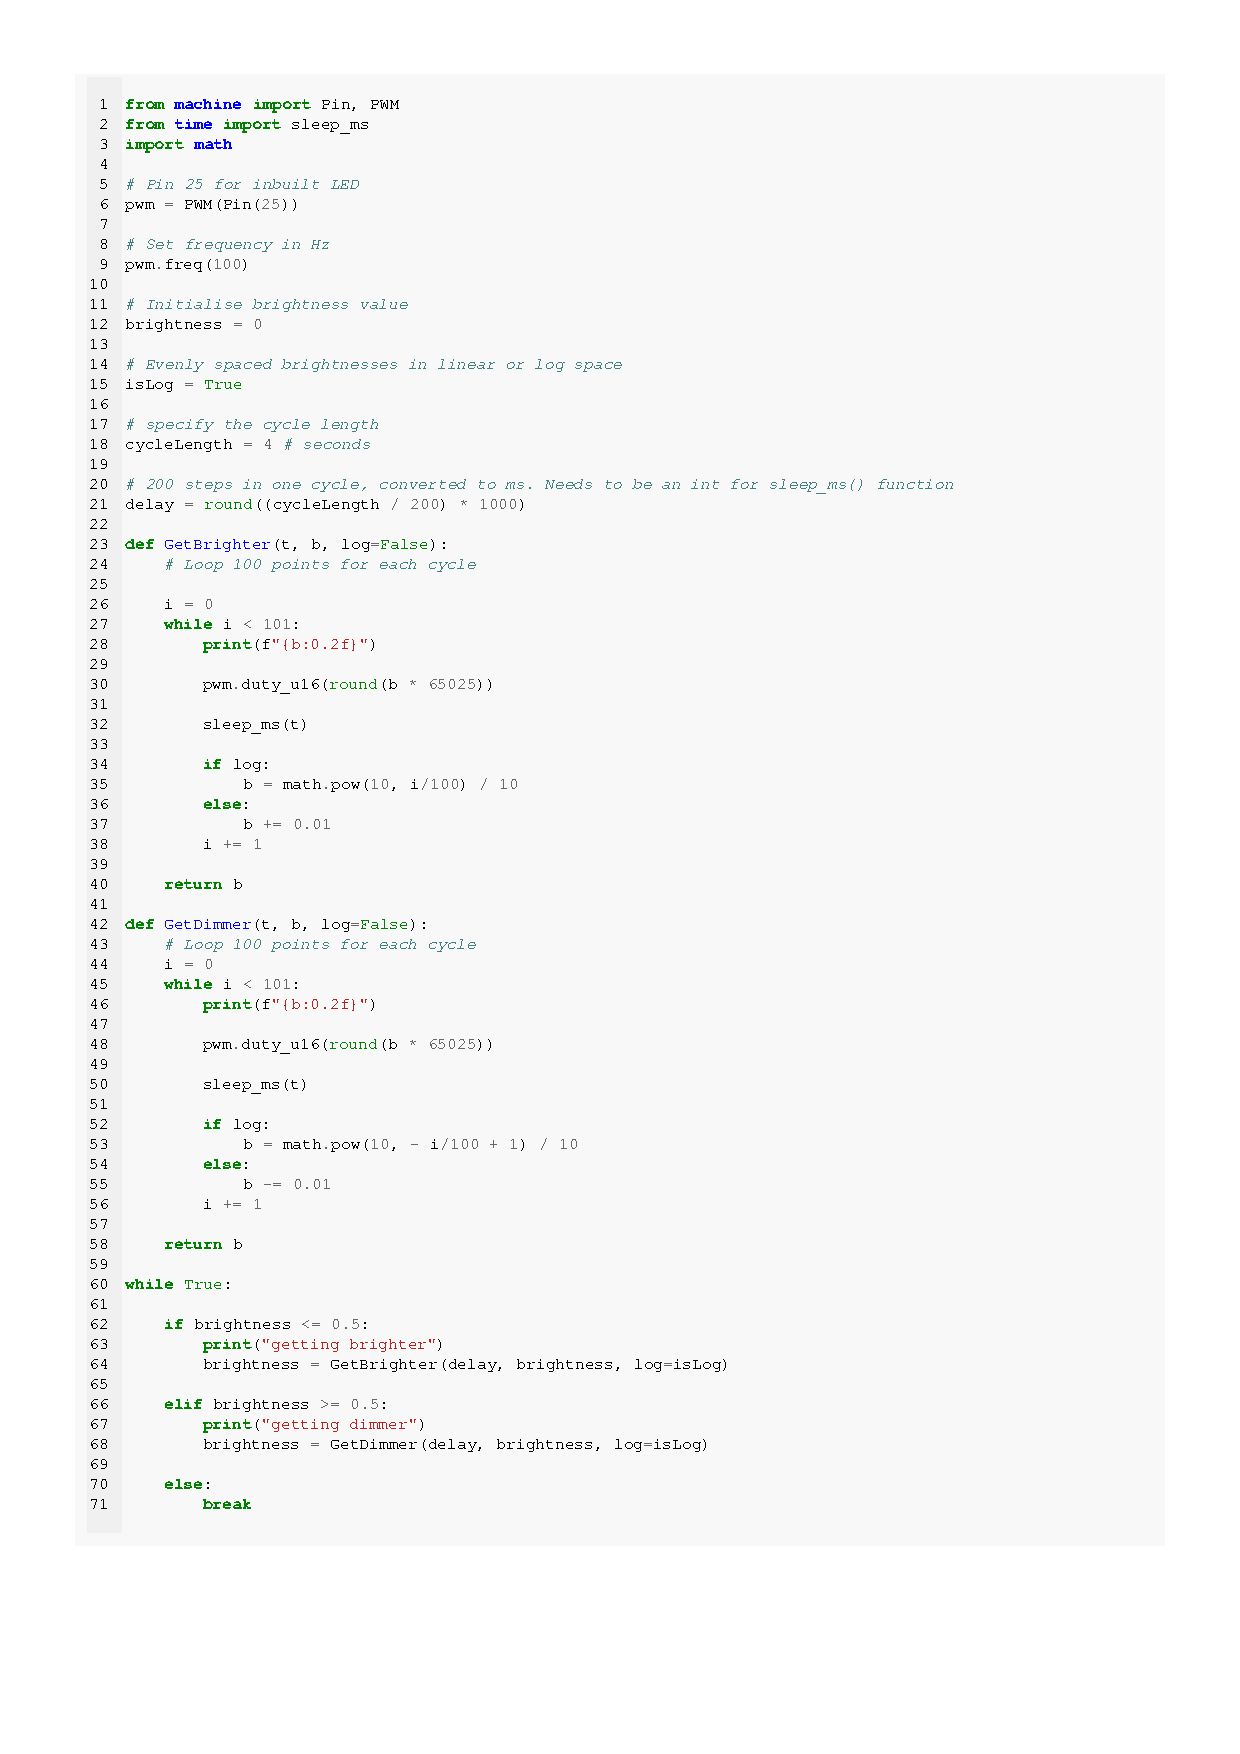
\includegraphics[width=\columnwidth]{Images/linearLogBrightness.pdf}
    \end{figure}

\clearpage

\section{Function Generator Script}
    \begin{figure}[h]
        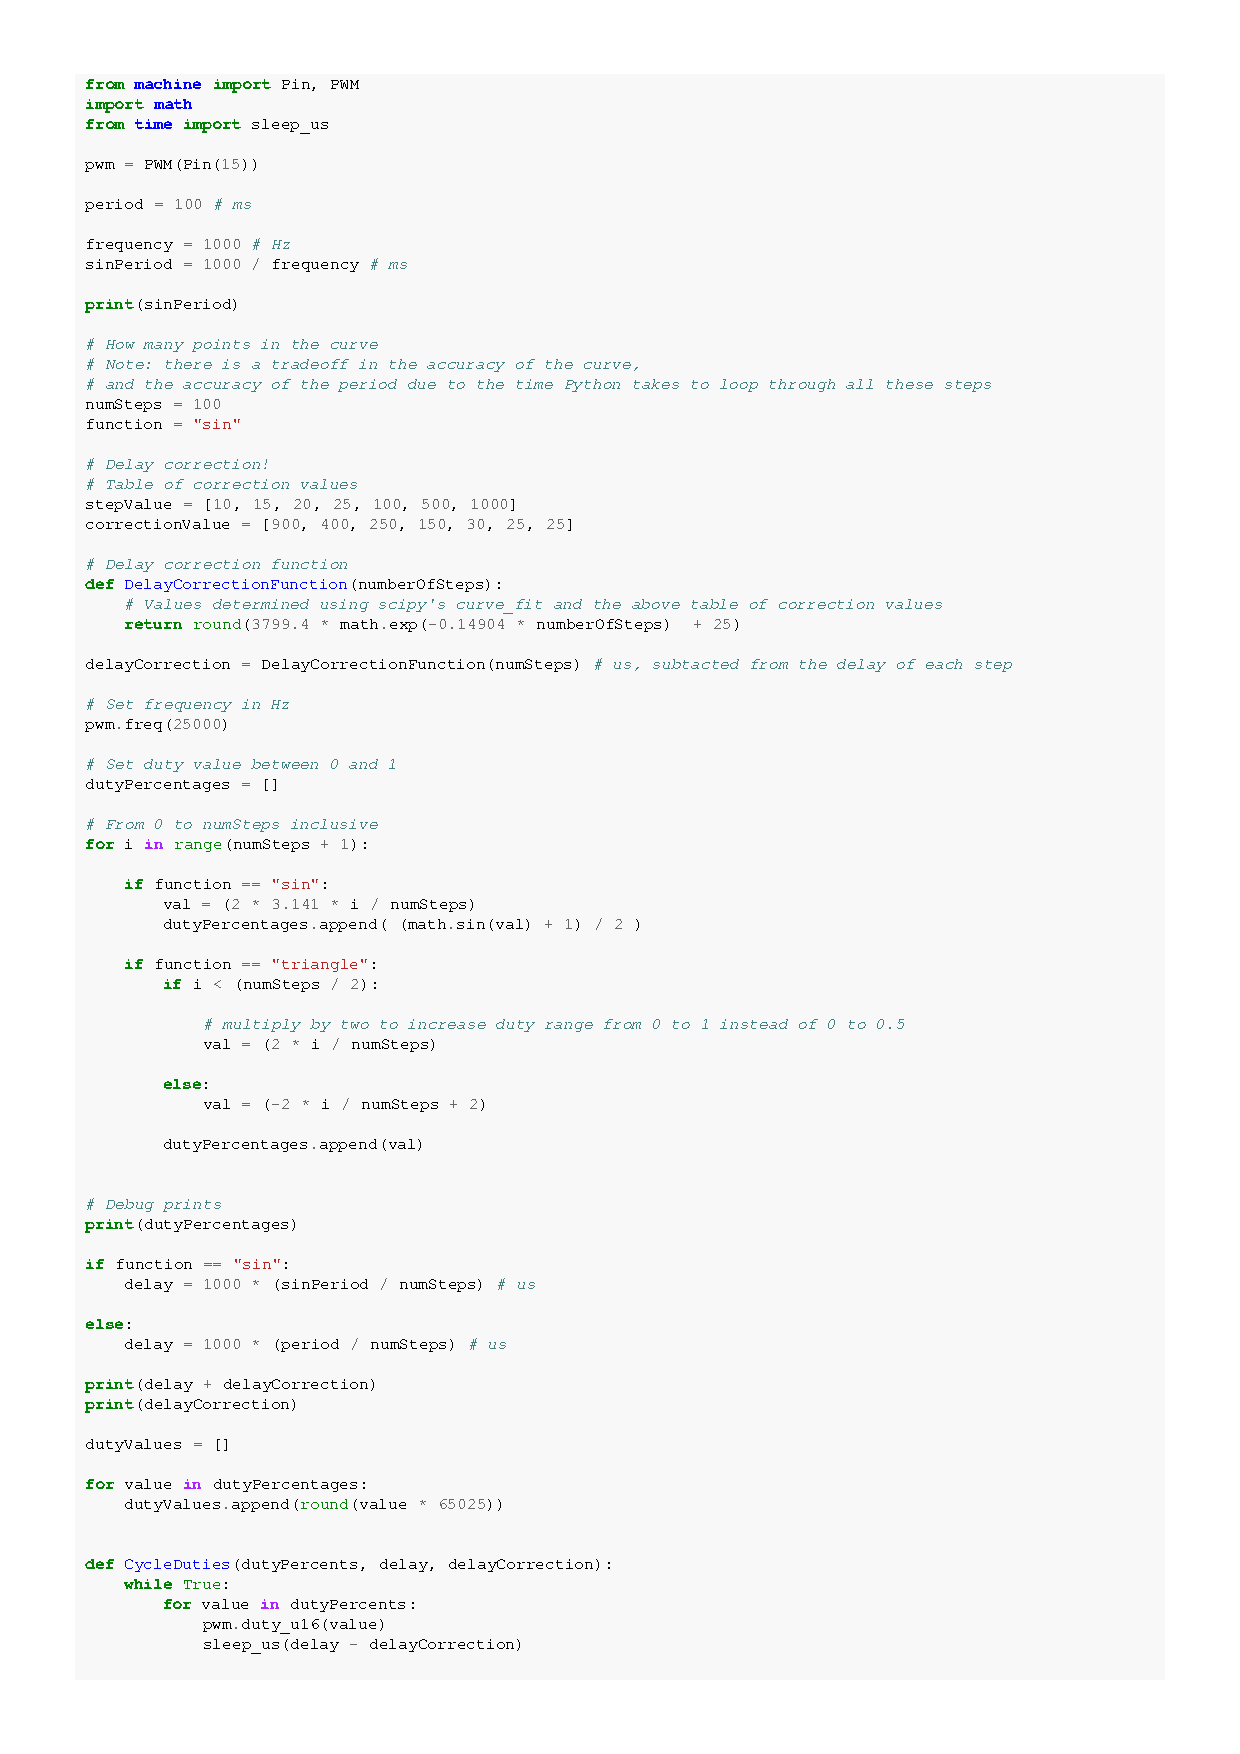
\includegraphics[width=\columnwidth,page=1]{Images/functionGenerator.pdf}
    \end{figure}
    \begin{figure}[h]
        \includegraphics[width=\columnwidth,page=2]{Images/functionGenerator.pdf}
    \end{figure}

\clearpage
\section{Python Analysis Notebooks}
    

\end{document}
%
% ****** End of file apssamp.tex ******
